\documentclass[10pt]{article}
\usepackage{icmlko}

\icmlmeta{IP 파운데이션 월드모델}{341}{쌍둥이 검사}{축이 제 섞은 쌍둥이를 이기나 --- 검사를 만들고, 그 답으로 축을 뺐더니 안 올랐다}

\begin{document}

\twocolumn[
\icmlheader

\begin{abstract}
노트 340이 ``채택의 문턱은 0 보다 나은가가 아니라 제 섞은 쌍둥이보다
나은가''로 끝났다. \textbf{검사 다섯째를 만들었다}
(\texttt{lab/scrambled.py}) --- 축의 \emph{관측된 값끼리만} 섞어 열 수 ·
관측 무늬 · 결측 자리를 그대로 두고 정보만 없앤 쌍둥이를 만들고,
\textbf{같은 학습 재추출 뽑기에서} 둘을 견준다.

위키 계열에 돌렸다(노트 340에서 $-$0.0070 으로 제일 얇게 벌던 계열).

\begin{center}\footnotesize
\begin{tabular}{lrr}
\hline
도메인 & 진짜 $-$ 쌍둥이 & 양수 \\
\hline
\textbf{세계애니} & \textbf{$+$0.0584} & \textbf{8/8} \\
게임 & $+$0.0102 & 7/8 \\
\textbf{시장팝업} & \textbf{$-$0.0873} & \textbf{0/8} \\
\textbf{애니} & $-$0.0070 & \textbf{0/8} \\
\hline
판 & $+$0.0024 & 6/8 \\
\hline
\end{tabular}
\end{center}

\textbf{네 도메인이 갈렸다} --- 세계애니와 게임에서는 진짜가 이기고,
시장팝업과 애니에서는 \textbf{제 잡음보다 못하다.} 넷 중 어느 것도
검사 ①$\sim$④ 로는 안 나오는 답이다(그 넷은 도메인별 답을 안 준다).

\textbf{그래서 진 둘에서 위키를 뺐다. 안 올랐다.} 판
$+$0.0009(SD 0.0038 · 7/12) --- 미결정 폭 안이다. 그리고 시장팝업 자체가
\textbf{기준 한 번으로는 $+$0.0347} 인데 짝지으면 0.002 아래다.
\textbf{노트 338의 덫에 또 걸릴 뻔했다.}

\textbf{그러므로 검사 ⑤ 는 ``붙일까''에 답하지 ``뺄까''에는 답하지 않는다.}
노트 340이 이미 그 비대칭을 봤다 --- 잡음 축을 \emph{붙이면} $-$0.126
인데 실제 계열을 \emph{빼면} $-$0.007$\sim$$-$0.044 다. \textbf{붙이기와
빼기는 서로의 역이 아니다.}
\end{abstract}
]

\section{검사 다섯째}

\begin{center}\footnotesize
\begin{tabular}{ll}
\hline
검사 & 무엇을 묻나 \\
\hline
① 학습 상관 & 정보가 있나 \\
② 시간 조각 & 시기에 안 흔들리나 \\
③ 겹침 & 새로운가 \\
④ 비상수성 & 갈라 주나 \\
\textbf{⑤ 쌍둥이} & \textbf{제 잡음보다 나은가} \\
\hline
\end{tabular}
\end{center}

\textbf{①$\sim$④ 는 다 학습 구간에서 축이 무엇을 아는가를 잰다.} ⑤ 만
유보를 본다 --- 그래서 싸지 않다(뽑기마다 적합이 둘, 여덟 뽑기면 열여섯
번). 다른 이름표처럼 매 실행에 자동으로 안 붙이고 \textbf{축을 붙일지
정하는 날 한 번 부른다.}

\begin{figure*}[t]
\centering
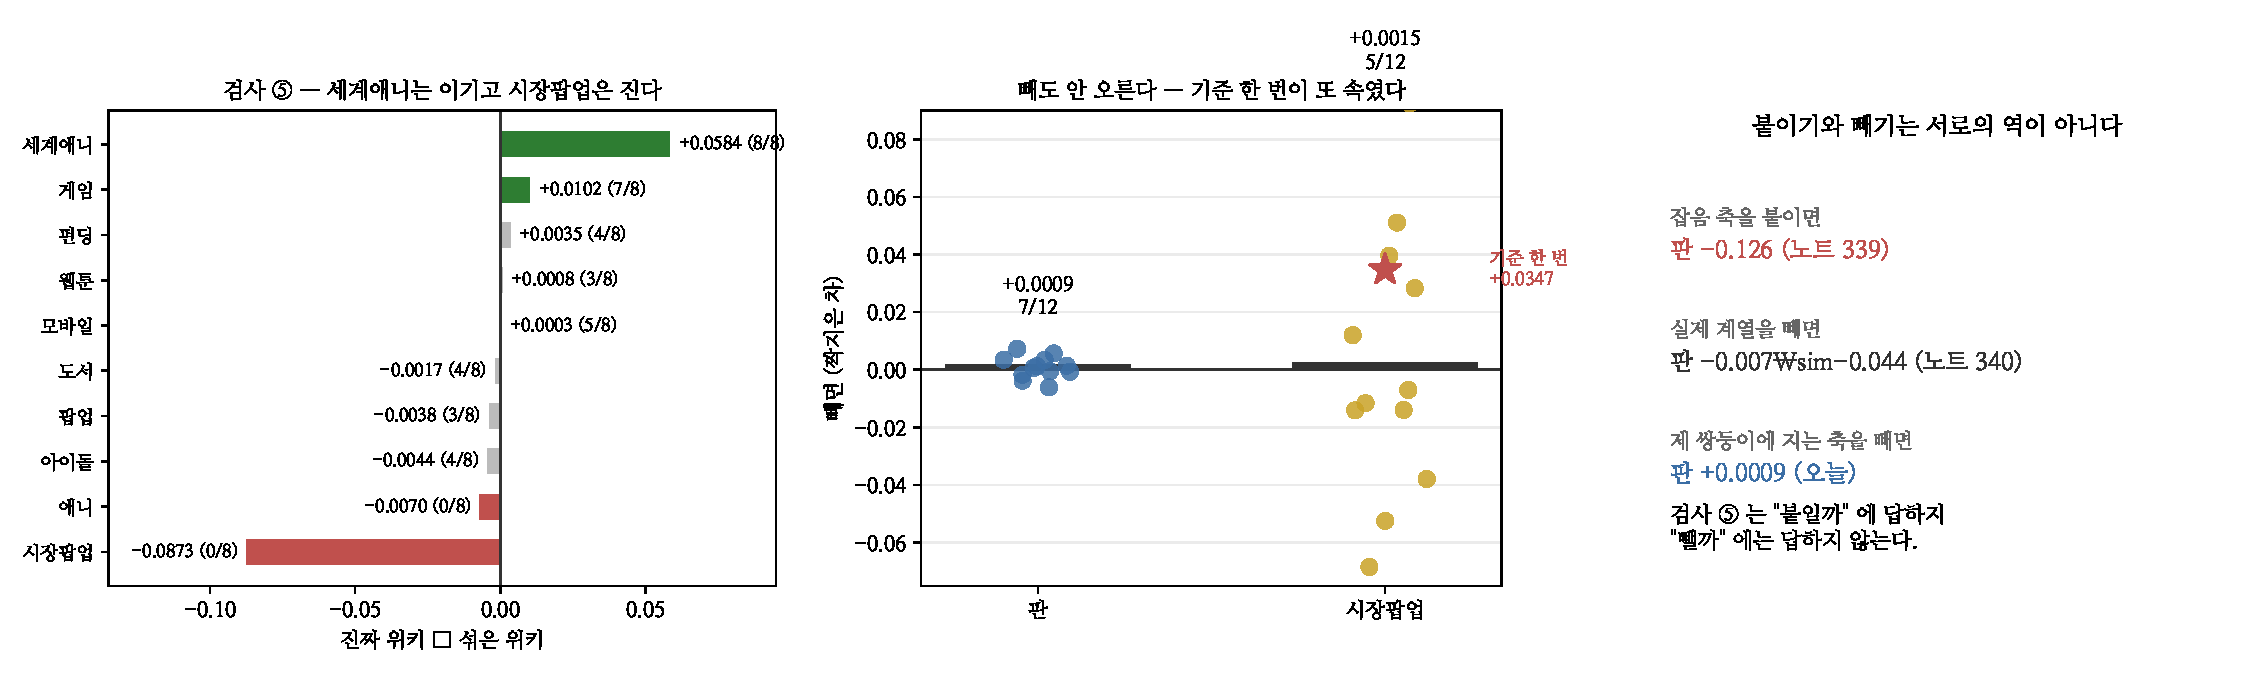
\includegraphics[width=\textwidth]{figs/twins.pdf}
\caption{왼쪽 --- 검사 ⑤ 의 도메인별 답. 가운데 --- 진 둘에서 빼 보면.
오른쪽 --- 붙이기와 빼기의 비대칭.}
\end{figure*}

\section{위키 계열에 돌렸다}

\begin{center}\footnotesize
\begin{tabular}{lrrl}
\hline
도메인 & 차 & 양수 & 덮음 \\
\hline
세계애니 & $+$0.0584 & 8/8 & 55\% \\
게임 & $+$0.0102 & 7/8 & 49\% \\
펀딩 & $+$0.0035 & 4/8 & 0.5\% \\
웹툰 & $+$0.0008 & 3/8 & 12\% \\
모바일 & $+$0.0003 & 5/8 & 11\% \\
도서 & $-$0.0017 & 4/8 & 21\% \\
팝업 & $-$0.0038 & 3/8 & 60\% \\
아이돌 & $-$0.0044 & 4/8 & 82\% \\
애니 & $-$0.0070 & \textbf{0/8} & 36\% \\
시장팝업 & $-$0.0873 & \textbf{0/8} & 38\% \\
\hline
\end{tabular}
\end{center}

\textbf{덮음으로는 안 설명된다} --- 아이돌은 82\%인데 $-$0.0044 이고
게임은 49\%인데 $+$0.0102 다. \textbf{세계애니만 크게 이긴다}(문서 있음
1,624건 · 창 채움 1,296건으로 절대량이 제일 크다).

\section{빼 봤더니 안 올랐다}

\begin{center}\small
\begin{tabular}{lrr}
\hline
 & 기준 한 번 & 짝지어 열둘 \\
\hline
판 & $+$0.0012 & $+$0.0009 (7/12) \\
\textbf{시장팝업} & \textbf{$+$0.0347} & \textbf{$<$0.002} \\
애니 & $-$0.0002 & $+$0.0037 (7/12) \\
\hline
\end{tabular}
\end{center}

\textbf{시장팝업의 $+$0.035 가 짝지으면 사라진다.} 노트 338이 ``차이도
한 번 재면 안 된다''를 세운 뒤 \emph{처음으로} 그 규약이 실제로 막아
준 자리다 --- 기준값만 봤으면 ``검사 ⑤ 가 맞혔다''고 썼을 것이다.

\paragraph{덤} 손 안 댄 팝업이 $+$0.0236(11/12)로 올랐다. 노트 329가
잰 통로다 --- \textbf{남의 열을 빼면 내 점수가 움직인다.}

\section{왜 안 오르나}

\begin{center}\footnotesize
\begin{tabular}{lr}
\hline
잡음 축을 \textbf{붙이면}(노트 339) & 판 $-$0.126 \\
실제 계열을 \textbf{빼면}(노트 340) & 판 $-$0.007$\sim$$-$0.044 \\
쌍둥이에 지는 축을 \textbf{빼면}(오늘) & 판 $+$0.0009 \\
\hline
\end{tabular}
\end{center}

섞기는 열을 \emph{남겨 두고} 정보만 없앤다. 빼기는 열을 \emph{치운다}.
\textbf{나무한테 그 둘은 다른 사건이다} --- 남은 잡음 열은 갈림을
훔치지만, 치운 열은 아무 일도 안 한다. \textbf{그래서 ``제 잡음보다
못하다''가 ``없는 편이 낫다''를 뜻하지 않는다.}

\section{남은 것}
\begin{center}\footnotesize
\begin{tabular}{ll}
\hline
갈래 & 왜 \\
\hline
\textbf{검사 ⑤ 를 붙이기 전에} & 새 축 후보에 돌려 보라 \\
세계애니 위키 $+$0.058 & 유일하게 크게 이긴다 \\
빼기 검사를 따로 & ``없는 편이 나은가''는 다른 물음 \\
팝업이 왜 $+$0.024 인가 & 손 안 댔는데 올랐다 \\
\hline
\end{tabular}
\end{center}

\paragraph{규약} \textbf{검사를 만들면 그 검사가 무엇에 답하는지도 재야
한다.} 노트 340이 ``제 쌍둥이보다 나은가''를 채택 문턱으로 제안했고 오늘
그 검사를 만들었는데, 만들고 나서 \emph{그 답으로 무엇을 할 수 있나}를
재 보니 \textbf{빼기에는 못 쓴다.} 검사는 맞았고 쓰임새를 내가 넓게
잡았다. \textbf{도구를 만든 날 그 도구의 경계도 같이 재라} --- 안 그러면
다음 노트가 그 경계를 모르고 쓴다.

\end{document}
